\documentclass{beamer}
% \documentclass[handout]{beamer}

\batchmode
\usepackage{amsmath,amssymb,enumerate,epsfig,bbm,calc,color,ifthen,capt-of,etoolbox,hyperref,lmodern}
\usepackage[backend=bibtex,citestyle=numeric]{biblatex} %use biblatex package for references
\addbibresource{references.bib}          %Load bibliography .bib file

\usetheme{Berlin}                        %use Berlin as theme
\usecolortheme{tigers}                   %use tigers as colortheme

\makeatletter                            %resize header in Berlin theme to match a header with no circles
\setbeamertemplate{headline}
{%
  \begin{beamercolorbox}[colsep=1.5pt]{upper separation line head}
  \end{beamercolorbox}
  \begin{beamercolorbox}{section in head/foot}
    \vskip2pt\insertsectionnavigationhorizontal{\paperwidth}{}{}\vskip2pt
  \end{beamercolorbox}%
  \ifbeamer@theme@subsection%
    \begin{beamercolorbox}[colsep=1.5pt]{middle separation line head}
    \end{beamercolorbox}
    \begin{beamercolorbox}[ht=2.5ex,dp=1.125ex,%
      leftskip=.3cm,rightskip=.3cm plus1fil]{subsection in head/foot}
      \usebeamerfont{subsection in head/foot}\insertsubsectionhead
    \end{beamercolorbox}%
  \fi%
  \begin{beamercolorbox}[colsep=1.5pt]{lower separation line head}
  \end{beamercolorbox}
}
\makeatother

\makeatletter            %reduce spacing between section entries in table of contents
\patchcmd{\beamer@sectionintoc}{\vskip1.5em}{\vskip1.0em}{}{}
\makeatother

%define title page
\title{Topic 2-1: Likelihood Construction and Estimation}
\subtitle{Univariate Models}
\author{}
\institute{Department of Experimental Statistics, Louisiana State University}
\date{July 25, 2021}
\pgfdeclareimage[height=0.5cm]{lsu-logo}{./images/lsu-logo.png}
\logo{\pgfuseimage{lsu-logo}\hspace*{0.3cm}}

\AtBeginSection[]        %the table of contents will appear before each section
{
  \begin{frame}<beamer>
      \frametitle{Contents}
      \tableofcontents[currentsection, hideothersubsections]
  \end{frame}
}
\beamerdefaultoverlayspecification{<+->}

%begin the document
\begin{document}
%------Title------%
\frame{\titlepage}

%------Acknowledgement------%
\begin{frame}{Content}
    \vspace{1ex}
Discrete IID Random Variables\\
Multinomial Likelihoods\\
Continuous IID Random Variables\\
Mixtures of Discrete and Continuous Components\\
Proportional Likelihoods\\
The Empirical Distribution Function as an MLE\\
Likelihoods from Censored Data
\end{frame}

%------Table of Contents------%
\begin{frame}{Contents}
    \tableofcontents[hidesubsections]
\end{frame}

%------Introduction------%
\begin{section}{Introduction}                   %SECTION 'Introduction'
    \subsection{Problem Statement}              %subsection 1
    \begin{frame}{Problem Statement}
        \begin{itemize}
            \item
            \item
            \item
        \end{itemize}
    \end{frame}

    \subsection{Importance of the Research}     %subsection 2
    \begin{frame}{Importance of the Research}
        \begin{itemize}
            \item
            \item
            \item
        \end{itemize}
    \end{frame}
    \end{section}

%------Literature Review------%
\begin{section}{Literature Review}              %SECTION 'Literature Review'
    \subsection{Prior Work}                     %subsection 1
    \begin{frame}{Prior Work}
        \begin{itemize}
            \item MapReduce\cite{dean2008mapreduce}
            \item AlphaGo\cite{silver2016mastering}
            \item
        \end{itemize}
    \end{frame}

    \subsection{Limitation}                     %subsection 2
    \begin{frame}{Limitation}
        \begin{itemize}
            \item
            \item
        \end{itemize}
    \end{frame}
\end{section}

%------Research Questions------%
\begin{section}{Research Questions}             %SECTION 'Research Questions'
    \begin{frame}{Research Questions}
        \begin{itemize}
            \item
            \item
        \end{itemize}
    \end{frame}
\end{section}


%------Study Area and Data------%
\begin{section}{Study Area and Data}           %SECTION 'Study Area and Data'
    \subsection{Study Area}                    %subsection 1
    \begin{frame}{City and County of San Francisco}
        \begin{columns}[T]
            \column{0.7\textwidth}<1->
                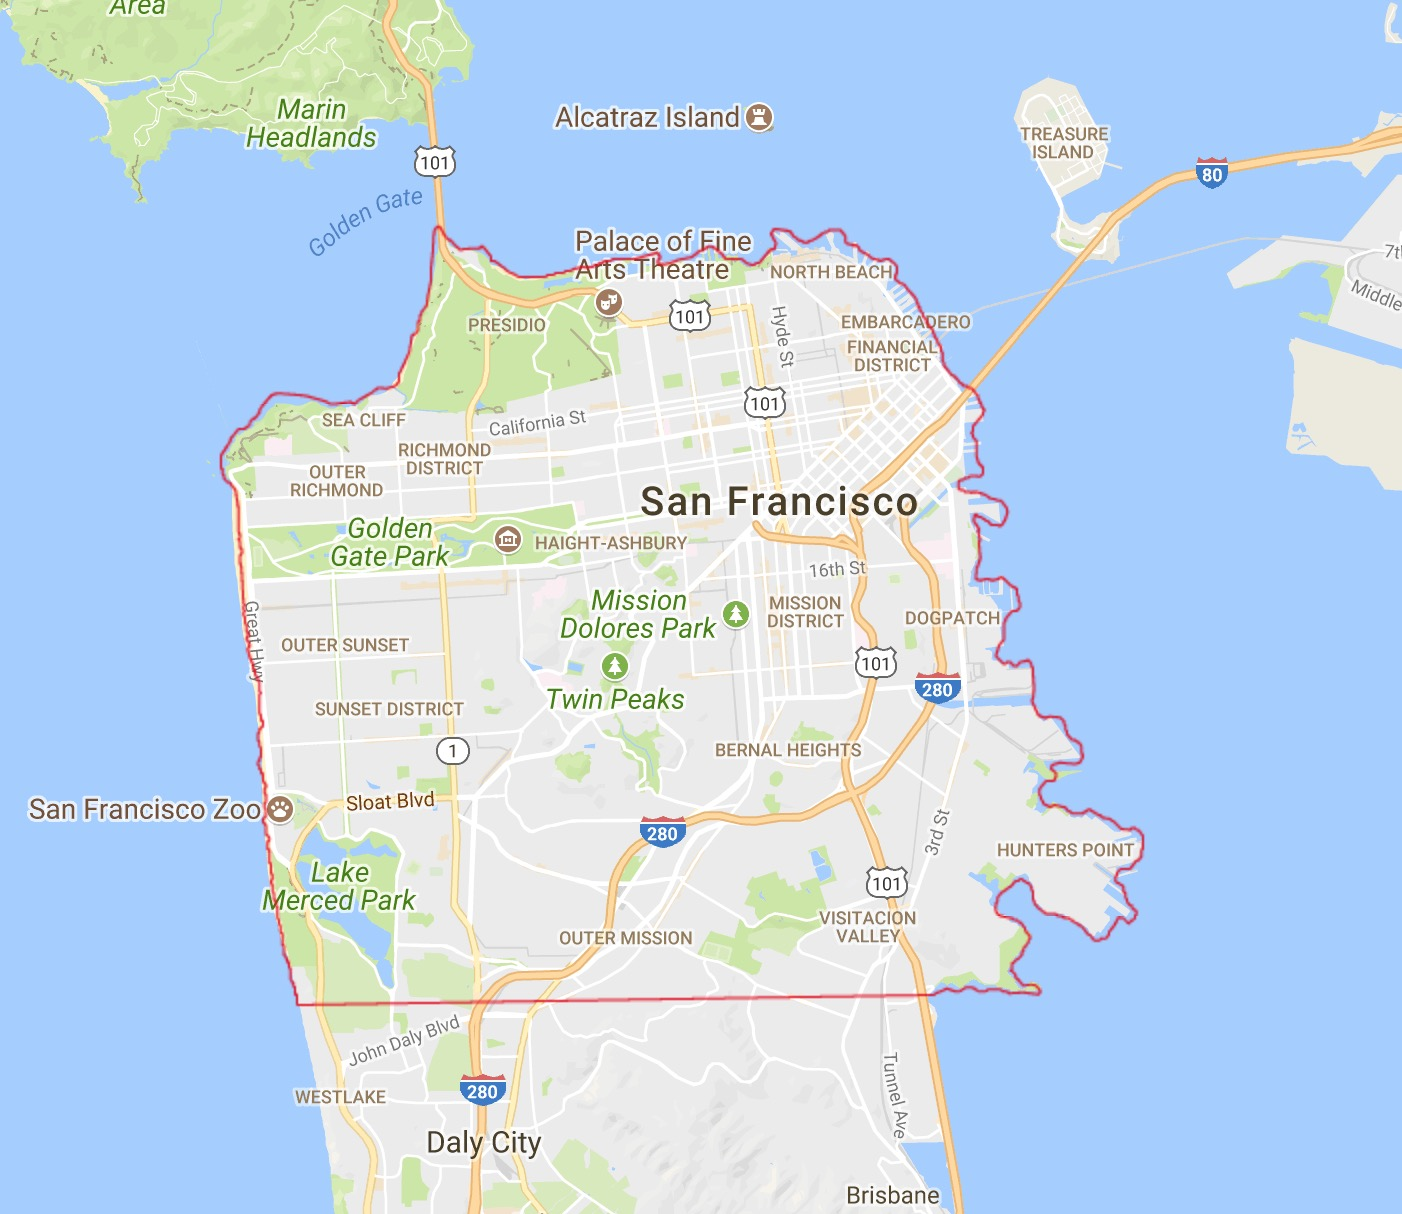
\includegraphics[width=\linewidth]{./images/sanfrancisco.jpg}
            \column{0.4\textwidth}
                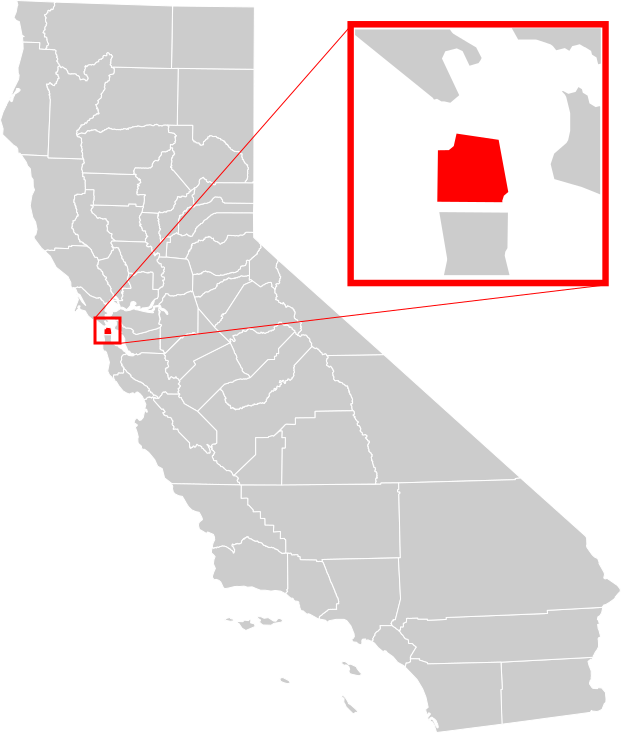
\includegraphics[width=0.7\linewidth]{./images/california-sanfrancisco.png}
                \vskip 1em
                \begin{itemize}
                    \item \scriptsize{Population: 864,816 (2015)}
                    \item \scriptsize{Land Area: 46 $mi^2$}
                \end{itemize}
        \end{columns}
    \end{frame}

    \subsection{Data}                           %subsection 2
    \begin{frame}{Datasets}
        \begin{columns}
        \setbeamercovered{transparent}
            \column{0.5\textwidth}
                \begin{block}{Dataset 1}<1->
                    \begin{itemize}
                        \item
                        \item
                    \end{itemize}
                \end{block}
                \begin{block}{Dataset 2}
                    \begin{itemize}
                        \item
                        \item
                    \end{itemize}
                \end{block}

            \column{0.5\textwidth}
                \begin{block}{Dataset 3}
                    \begin{itemize}
                        \item
                        \item
                    \end{itemize}
                \end{block}
                \begin{block}{Dataset 4}
                    \begin{itemize}
                        \item
                        \item
                    \end{itemize}
                \end{block}
        \setbeamercovered{invisible}
        \end{columns}
    \end{frame}
\end{section}

%------Methodology------%
\begin{section}{Methodology}                     %SECTION 'Methodology'
    \subsection{Design of Framework}             %subsection 1
    \begin{frame}{Design of Framework}
        \begin{itemize}
            \item
            \item
            \item
        \end{itemize}
    \end{frame}

    \subsection{Trainging}                       %subsection 2
    \begin{frame}{Training}
        \begin{itemize}
            \item
            \item
            \item
        \end{itemize}
    \end{frame}

    \subsection{Validation}                      %subsection 3
    \begin{frame}{Validation}
        \begin{itemize}
            \item
            \item
            \item
        \end{itemize}
    \end{frame}
\end{section}

%------References------%
\begin{frame}{References}
    \printbibliography
\end{frame}

%------Thanks------%
\begin{frame}{}
    \begin{center}
    \huge{Thanks!}
    \end{center}
\end{frame}

\end{document}
